\chapter{Sorting and searching algorithms}

\begin{goals}
% \item Understand why designing efficient algorithms is important and how to measure algorithms' performance
\item Understand what sorting and searching are and why they are important
\item Understand what insertion sort is
\item Understand linear search and binary search
\item Learn how to code these algorithms in Java
\end{goals}

%  \section{Algorithm analysis}
 
%  We will start off this chapter by building an intuitive understanding of why different implementations of the same algorithm have different performance (running time). We will first discuss how to observe and model performance characteristics of algorithms and then discuss how we can classify the algorithms based on the order of growth of their running time. 

% Understanding how to compare the performance of different algorithms and provide guarantees on how well they perform will help us learn and compare the sorting and searching algorithms we will be considering later in this chapter. 


% The main reason we would like to have a sense of the performance of an algorithm is to be able to tell whether the program can solve a large practical input or not. Given two computer programs that perform the same task, how can we tell which program is 'faster'? The most straightforward way is to time each program, for example, using the stopwatch. However, here, we assume that the two programs are run on the same computer to make the comparison fair. We can not make a meaningful comparison of the two programs if we ran them on different computers because even running the same programs on two different computers would likely lead to two different running times since one computer might have a better hardware (processor speed, memory, disk space). 

% Therefore, this way of measuring the performance of an algorithm is not the most convenient one. Another way of measuring the performance independent of the type of computer we use is by counting the number of instructions or operations in the two programs. Usually, the faster program has fewer operations. Intuitively, we would also expect that the number of operations is proportional to the number of data items that the program operates on. 



% Donald Knuth pioneered the following approach to understating the total running time of a program:

% Total running time: sum of cost $\times$ frequency of all operations.

% Therefore, we need to analyze a program to determine the set of operations it uses. The cost depends on the machine and the compiler. The frequency of the operations depends on the algorithm as well as input data. 

% \begin{exercise}
% \begin{code}
% int count = 0;
% for (int i = 0; i < N; i++)
% 	If (a[i] == 0)
% 		count++;
% \end{code}

% For each operation (variable declaration, assignment statement, less than compare, equal compare, array access, increment), determine its frequency of execution as a function of input size $N$.

% \end{exercise}



% Though, in theory, we could determine the running time of a program using Donald Knuth’s method, we usually don’t need to know the running time with such precision. We can approximate the running time by making the following simplifications: 1) use some basic operation (perhaps the one that costs the most) as a proxy for running time; 2) only consider the highest order terms in our derivation of the running time. For example, if we derived the running time to be $\frac{1}{2}N^3 + 50 N$, we would approximate this with ~ $\frac{1}{2}N^3$.

% Next, it turns out that the following set of functions 
% $1, logN, N, NlogN, N^2, N^3, 2^N$
% suffices to describe order-of-growth of typical algorithms. 


\section{Introduction to Sorting and Searching}

Sorting and searching are central tasks in programming -- they are so fundamental that you are probably familiar with them already. For example,have ever been in a group of people and lined up by increasing order of height? If so, then you have engaged in \emph{sorting}, or putting items in a specific order based on their attributes. As another example, have you ever looked through a deck of cards for a specific card? Or maybe you've looked through a phone book for someone's phone number? If so, then you've engaged in \emph{searching}, or looking for an item with a specific attribute. 
Sorting and searching are tasks you do every day, sometimes without even thinking about it! 

Searching and sorting are also important in programming. For example, in your Java code files, you can search for all occurrences of a word in the code in order to replace it with another word (try it!). You can also sort files on your computer into alphabetical order based on the first character of the file's name. Because searching and sorting are common and important computer tasks, programmers in the past have spent a lot of time developing fast methods, or \emph{algorithms}, for sorting and searching. In this chapter, we'll discuss what it means to develop a sorting or searching algorithm, and go into the code behind some of these methods.

\section{Sorting algorithms}

Although sorting appears in many different contexts, these problems often reduce down to the same problem: given an array of numbers, return an array with the numbers in order from least to greatest. For example, consider the following \ic{int} array:
\begin{code}
int[] myArray = {4, 3, 2, 10, 12, 1, 5, 6};
\end{code}
Then, sorting \ic{myArray} would mean returning an array \ic{mySortedArray} that looks like
\begin{code}
int[] mySortedArray = {1, 2, 3, 4, 5, 6, 10, 12};
\end{code}

Despite the simplicity of the sorting problem, many algorithms have been developed over the years for sorting arrays. To give you a sense of how many sorting algorithms there are, the Wikipedia page for ``sorting algorithms" contains over 25 of them! Some popular sorting algorithms that you might here include quicksort, mergesort, bubble sort, and heap sort. There's even a sorting algorithm called ``timsort", named after a programmer named Tim Peters. In this section, we will go over a sorting algorithm called \emph{insertion sort}.

 \begin{figure}
    \centering
    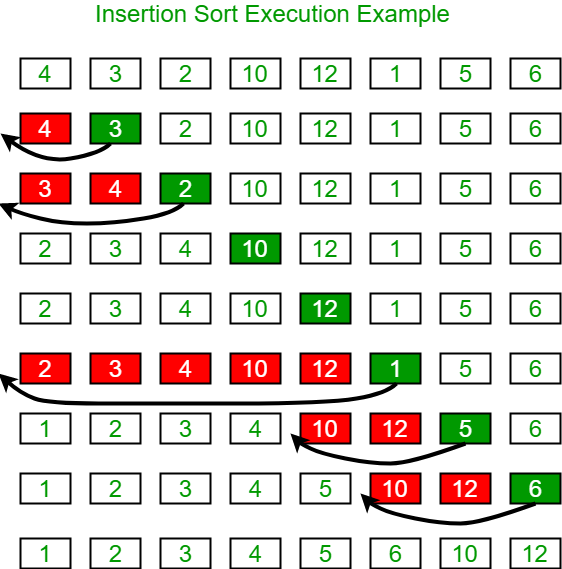
\includegraphics[width=0.7\textwidth]{images/insertionsort.png}
    \caption{An example showing how the insertion sort algorithm works.}
    \label{fig:insertion_sort}
\end{figure}


\subsection{Insertion Sort}

Insertion sort is a sorting algorithm that is based on how people tend to sort hands of playing cards. The insertion sort algorithm works as follows.
\begin{enumerate}
 \item Look at entries $0, 1$ of the array. Move entry $0$ backwards if it is smaller than the first entry.
 \item Look at entries $0, 1, 2$ of the array. Move entry $2$ backwards until it is in the right spot (i.e. entries $0,1,2$ are in sorted order).
 \item Look at entries $0, 1, 2, 3$ of the array. Move entry $2$ backwards until it is in the right spot (i.e. entries $0,1,2, 3$ are in sorted order).
 \item Look at entries $0, 1, 2, 3, 4$ of the array. . .
\end{enumerate}
 
We illustrate the insertion sort process described above for \ic{myArray} in Figure \ref{fig:insertion_sort}, where each line corresponds to a different step of the above description. For example, in the third line of Figure \ref{fig:insertion_sort}, we look at entries $0, 1, 2$ of the array. These entries are $\{3, 4, 2\}$. We move entry $2$ (the 2 in the green box) backwards until entries $0, 1, 2$ are in sorted order. 

\begin{exercise}
Write out the steps for using insertion sort on the following arrays
\begin{code}
int[] myArrayTwo = {-1, 12, 5, 3, 15};
int[] myArrayThree = {5, 4, 3, 2, 1};
\end{code}
\end{exercise}
 
\subsection{Coding Insertion Sort}
 
Now that we have described the insertion sort algorithm, the next step is to write a method that implements insertion sort.

\begin{code}
public static void insertionSort(int arr[]) 
{
    // YOUR CODE HERE
}
\end{code}

The method takes as input an array called \ic{arr}. After the method is run, the goal is for the array \ic{arr} to be in sorted order.\footnote{Note that the method above has return type \ic{void}, which means that it has no output. As an exercise, you'll implement a method that does not have return type \ic{void}, i.e. the output of the method is a sorted array.}
 
The structure of the insertion sort algorithm suggests using a for-loop. Why? This is because we look at the entries $0,1$, then entries $0,1,2$, then entries $0,1,2,3$, and so on. That is, we look at entries $0, 1, ..., k$, where $k=1, 2, 3, \dots, $ This suggests using a for-loop, which loops over the elements $k=1, 2, 3,  ..., n-1$, where $n$ is the length of the array.

\begin{code}
void insertionSort(int arr[]) 
{
    int n = arr.length;
    for (int k = 1; k < n; k++) 
    {
        // YOUR CODE HERE
    }
}
\end{code}

\begin{exercise}
Why do we use \ic{k < n} in our loop instead of \ic{k <= n}? In other words, why do we not consider $k=n$?
\end{exercise}
 
Now let's think about what happens when we look at entries $0, 1, \dots, k$, for a fixed $k$. We take entry $k$ of \ic{arr}, i.e. \ic{arr[k]}, and keep moving it backwards until it is in the ``right" place.

We can implement this logic using a ``while" loop. Why? Because ``while" entry k is not in the right place, we move it backwards. Writing this out in pseudo-code, this roughly looks like the following.
 
\begin{code}
void insertionSort(int arr[]) 
{
    int n = arr.length;
    for (int k = 1; k < n; k++) 
    {
        while ( ENTRY k IS NOT IN THE RIGHT PLACE ) 
        {
            MOVE ENTRY k BACKWARDS;
        }
    }
}
\end{code}
 
However, there is one small catch: once we move the $k$-th entry backwards, then it is no longer the $k$-th entry! For example, in the second line of Figure \ref{fig:insertion_sort}, once we entry $1$ (i.e. the green square with a $3$) backwards once, it becomes entry $0$.

So to know the location of our original entry $k$, we will also define an additional variable, \ic{currentLoc}, which tells us the current location of entry k as we move it backwards.

 
\begin{code}
void insertionSort(int arr[]) 
{
    int n = arr.length;
    for (int k = 1; k < n; k++) 
    {
        int currentLoc = k;
        while ( arr[currentLoc] IS NOT IN THE RIGHT PLACE ) 
        {
            MOVE arr[currentLoc] BACKWARDS;
            currentLoc = currentLoc - 1;
        }
    }
}
\end{code}

Note that we initialize \ic{currentLoc=k}, since initially the $k$-th entry is at location $k$ (which makes sense!). We also include the line \ic{currentLoc = currentLoc - 1;} to account for moving \ic{arr[currentLoc]} backwards.

Let's finish the code by filling in our CAPITAL LETTERS. 

\textbf{Step 1: Coding the logic for ``\ic{arr[currentLoc] IS NOT IN THE RIGHT PLACE}"}. 

\ic{arr[currentLoc]} is in the right spot when both of the following are true:

\begin{enumerate}

 \item \textbf{We can't move \ic{arr[currentLoc]} any farther backwards, as it is at the beginning of the list.} For example, in line 6 of Figure \ref{fig:insertion_sort}, the green box $1$ is moved to the beginning of the list, as it cannot be moved any further backwards.
    \item \textbf{The entry to the left of \ic{arr[currentLoc]} is smaller than it and the entry to the right of \ic{arr[currentLoc]} is larger.} This means that \ic{arr[currentLoc]} is in its correct place. For example, in line 7 of Figure \ref{fig:insertion_sort}, the green box with a $5$ is in the right place when it is between $4$ and $10$, as $4$ is to the left of $5$ and $10$ is to the right of $5$. 
\end{enumerate}

The first case is written as \ic{currentLoc = 0}, and the second case is written as 
\begin{code}
arr[currentLoc] > arr[currentLoc - 1] && arr[currentLoc] < arr[currentLoc + 1]
\end{code}
\ic{arr[currentLoc]} is in the right spot if either the first case or the second case are true, i.e.

\begin{code}
currentLoc = 0 || (arr[currentLoc] > arr[currentLoc - 1] && arr[currentLoc] < arr[currentLoc + 1])
\end{code}

Thus, \ic{arr[currentLoc]} is \textbf{not} in the right spot if the negation of the above is true, i.e.
\begin{code}
!(currentLoc = 0 || (arr[currentLoc] > arr[currentLoc - 1] && arr[currentLoc] < arr[currentLoc + 1]))
\end{code}

So our pseudocode looks like


\begin{code}
void insertionSort(int arr[]) 
{
    int n = arr.length;
    for (int k = 1; k < n; k++) 
    {
        int currentLoc = k;
        while ( !(currentLoc = 0 || (arr[currentLoc] > arr[currentLoc - 1] && arr[currentLoc] < arr[currentLoc + 1])) ) 
        {
            MOVE arr[currentLoc] BACKWARDS;
            currentLoc = currentLoc - 1;
        }
    }
}
\end{code}
 
\textbf{Step 2: Coding the logic for ``\ic{MOVE \ic{arr[currentLoc]} BACKWARDS}"}. 
 
This step is equivalent to switching \ic{arr[currentLoc]} and \ic{arr[currentLoc- 1]} in the array. Assuming we have a method \ic{switch} for switching two entries in an array, our complete insertion sort code is as follows.

\begin{code}
void switch(int arr[], int i, int j) 
{
    // YOUR CODE HERE
}

void insertionSort(int arr[]) 
{
    int n = arr.length;
    for (int k = 1; k < n; k++) 
    {
        int currentLoc = k;
        while ( !(currentLoc = 0 || (arr[currentLoc] > arr[currentLoc - 1] && arr[currentLoc] < arr[currentLoc + 1])) ) 
        {
            switch(arr, currentLoc, currentLoc - 1);
            currentLoc = currentLoc - 1;
        }
    }
}
\end{code}

We leave the implementation of the \ic{switch} method as an exercise at the end of the chapter.

 
\section{Searching algorithms}

Similar to sorting, searching often reduces to the following problem: given an array \ic{arr} of numbers and a specific number $t$, return the index of $t$ in the array. For example, consider the following \ic{int} array:
\begin{code}
int[] myArray = {4, 3, 2, 10, 12, 1, 5, 6};
\end{code}
Then, if we are searching for $10$ in \ic{myArray}, we would want to return $3$, since $\ic{myArray[3]}$ is $10$.

Unlike sorting, there are not too many algorithms for searching in an array. If the array has no structure (e.g. it is totally random), then the only method is to do a \emph{linear search}, i.e. search through the array one-by-one. However, if the array is fully sorted, then we will discuss a faster algorithm for searching called \emph{binary search}.

  \begin{figure}
    \centering
    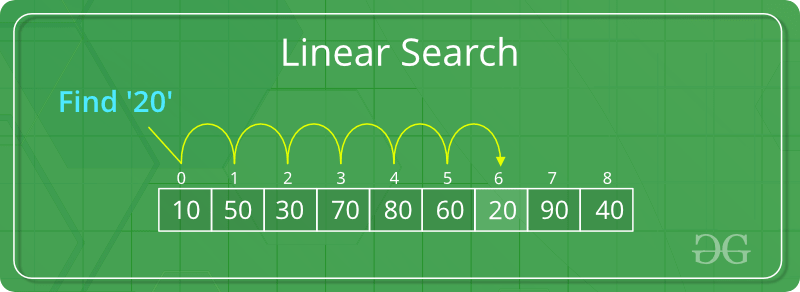
\includegraphics[width=0.9\textwidth]{images/Linear-Search.png}
    \caption{An example showing how the linear search algorithm works.}
    \label{fig:linear_search}
\end{figure}

\subsection{Linear Search}

Linear search consists of going through an array one entry at a time, until we find the item we are looking for. This is typically how people search through a list. For example, if you are given a list of numbers $\{1, 2, 3, 4, 5, 6\}$, and you are looking for the $6$, then you would go through the entries $1\dots 2\dots 3 \dots 4 \dots 5 \dots 6$ until you hit $6$.

Specifically, suppose you are given an array \ic{arr} and a entry \ic{t} to search for. Then in linear search, we do the following.
\begin{enumerate}
    \item Check if \ic{arr[0] == t}. If so, return 0.
    \item Check if \ic{arr[1] == t}. If so, return 1.
    \item Check if \ic{arr[2] == t}. If so, return 2.
    \item etc.
\end{enumerate}
 
As a concrete example, suppose our array looks like the following.
 \begin{code}
int[] myArrayThree = {10, 50, 30, 70, 80, 60, 20, 90, 40};
\end{code}
and we are searching for the entry 20. 

We first check if \ic{myArrayThree[0] == 20}. This is not true since \ic{myArrayThree[0]} is 10. So then we check if \ic{myArrayThree[1] == 20}. This is also not true since \ic{myArrayThree[1]} is 50. So then we check if \ic{myArrayThree[2] == 20}, and so on. We illustrate this process in Figure \ref{fig:linear_search}.

 
   \begin{figure}
    \centering
    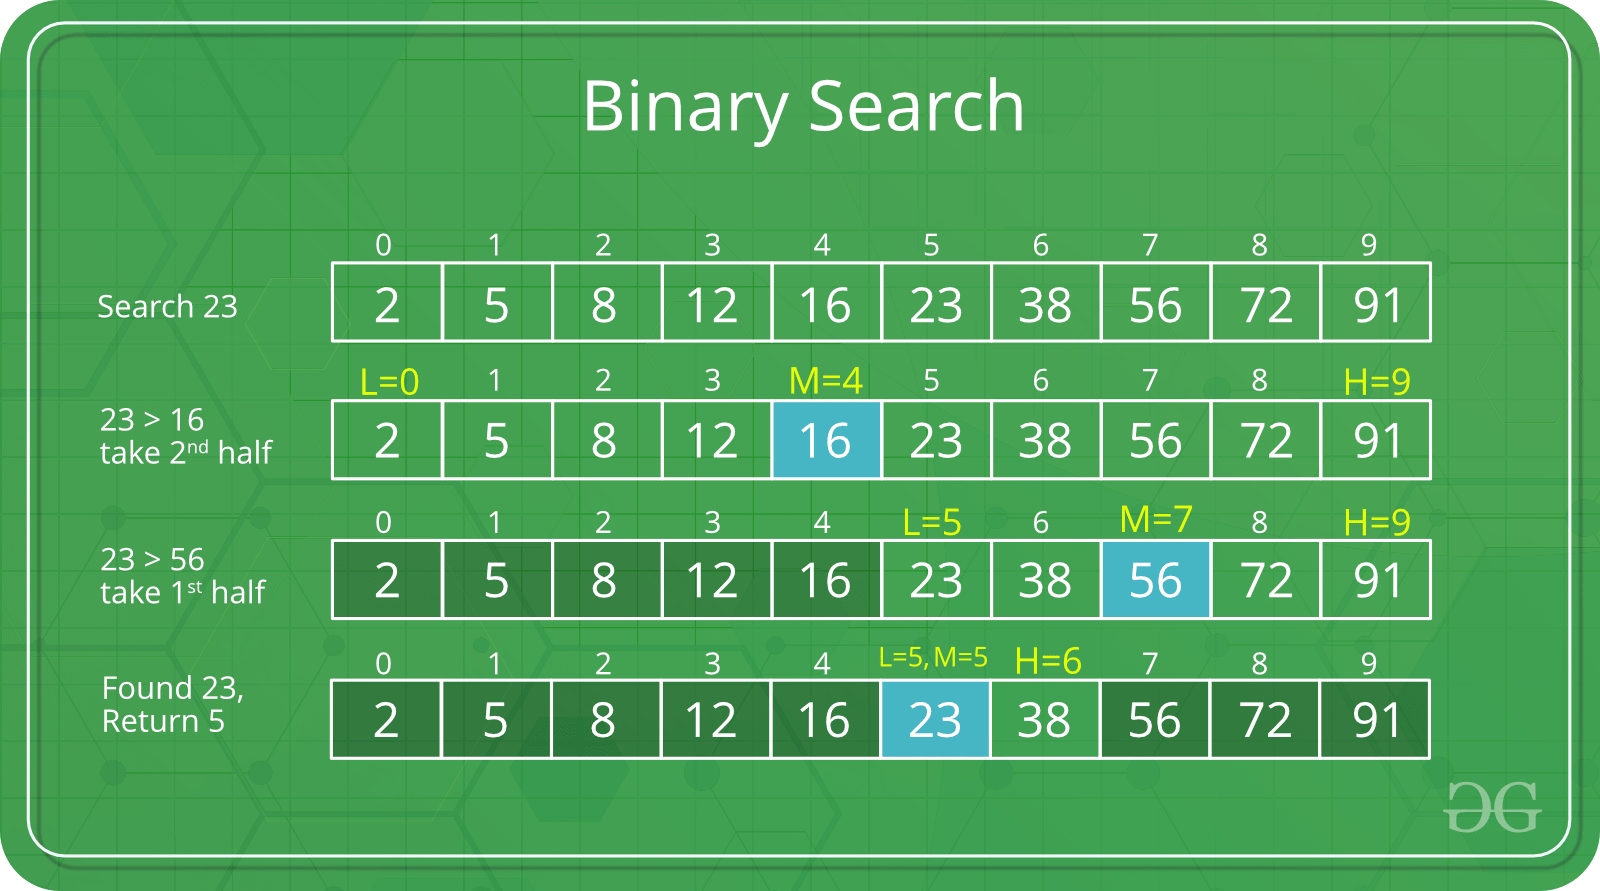
\includegraphics[width=0.9\textwidth]{images/Binary-Search.png}
    \caption{An example showing how the binary search algorithm works.}
    \label{fig:binary_search}
\end{figure}
 
 \subsection{Binary Search}
 On the other hand, if the array is sorted, then searching can be done more quickly by exploiting the fact that the array is already sorted. Let's look at an example.
 
 Suppose we have the following sorted array
 \begin{equation*}
     \{2, 5, 8, 12, 16, 23, 38, 56, 72, 91\}
 \end{equation*}
 and we are searching for the entry 23. 

Now say we look at the middle of the list, or 16. Because the array is sorted, we know that 23 has to be to the \emph{right} of 16 -- this is because everything to the left of 16 is smaller than 16, so 23 cannot be on the left.

\begin{equation*}
    \textcolor{red}{\{2, 5, 8, 12,} \textcolor{green}{16,} \textcolor{blue}{23, 38, 56, 72, 91\}}
\end{equation*}

Thus, we can completely ignore the left side of the array, i.e. $\textcolor{red}{2, 5, 8, 12}$ as we only need to search on the right side, i.e. $\textcolor{blue}{23, 38, 56, 72, 91}$. This eliminates searching half the array! 
% When the array is big, this is a huge improvement. For example, if the array had size 10000, then eliminating the left side of the array means we don't have to search 5000 entries. \footnote{In the project, we will explore how much this can speed-up your programs.}

So now we have reduced our problem to the following: given the array \ic{{23, 38, 56, 72, 91}}, search for the entry 23.
Once again, we can employ the same strategy. Look at the middle element of the list, or 56.

\begin{equation*}
    \textcolor{blue}{\{23, 38, } \textcolor{green}{56,} \textcolor{red}{72, 91\}}
\end{equation*}

Because 56 is larger than 23, the number we are searching for, we know that 23 has to be to the \emph{left} of 56. So we can ignore the right side $\textcolor{red}{72, 91}$ and only search for 23 in the left side $\textcolor{blue}{23, 38}$.

Once again, we repeat the same strategy. Here, because the array $\{23, 38\}$ has an even size, the middle of the array is either 23 or 38. If we pick the middle to be 23, then we have found the entry we are searching for, and we are done. Otherwise, we will have to repeat our ``look at the middle entry and eliminate half of the array" strategy one more time. For an illustration, see Figure \ref{fig:binary_search}.


This insight is the basic idea behind \emph{binary search}, a fast method for searching sorted arrays. At a high-level, binary search works as follows. Suppose you have an array \ic{int[] arr} and you are searching for an element \ic{t}. Then you do the following:

\begin{enumerate}
    \item Look at the middle entry \ic{arr[k]} of \ic{arr}, where \ic{k} is half of the size of \ic{arr}. For example, if \ic{arr} has size 11, then we would look at \ic{arr[5]}. (If the array has an even number of elements, pick either one of the middle elements.)
    \item Compare \ic{arr[k]} and t.
    \begin{itemize}
        \item If \ic{arr[k] = t}, then you found the element.
        \item Otherwise if \ic{arr[k] < t}, then ``throw out" the elements of \ic{arr} that are smaller than \ic{t}, i.e. everything to the left of \ic{t}.
        \item  Otherwise if \ic{arr[k] > t}, then ``throw out" the elements of \ic{arr} that are larger than \ic{t}, i.e. everything to the right of \ic{t}.
    \end{itemize}
    \item Repeat until \ic{arr} is a single entry. Then you have found your element.
\end{enumerate}

Let's look at another example. Suppose we are searching for the element 83 in the array

\begin{equation*}
    \{ 2, 3, 5, 7, 11, 13, 17, 19, 23, 29, 31, 37, 41, 43, 47, 53, 59, 61, 67, 71, 73, 79, 83, 89, 97   \}.
\end{equation*}

The middle entry of this array is 41, which is less than 83.

\begin{equation*}
    \textcolor{red}{\{ 2, 3, 5, 7, 11, 13, 17, 19, 23, 29, 31, 37,} \textcolor{green}{41,} \textcolor{blue}{43, 47, 53, 59, 61, 67, 71, 73, 79, 83, 89, 97   \}}.
\end{equation*}

Therefore, we can eliminate the left side of the array (red) and only look at the right side (blue):

\begin{equation*}
    \{43, 47, 53, 59, 61, 67, 71, 73, 79, 83, 89, 97\}.
\end{equation*}

Now we repeat. Because this array has an even size, the middle of this array is either 67 or 71. Let's pick 67.

\begin{equation*}
    \textcolor{red}{\{43, 47, 53, 59, 61,} \textcolor{green}{67,} \textcolor{blue}{71, 73, 79, 83, 89, 97   \}}.
\end{equation*}

The middle entry 67 is smaller than the entry we are looking for, 83. So we can eliminate the left side of the array (red), and only look at the right side (blue):

\begin{equation*}
    \{71, 73, 79, 83, 89, 97\}.
\end{equation*}

We repeat again. We divide the array at the middle entry, 79. (Note that depending on how we define ``middle", we could have instead picked 83 as the middle and finished our search.)

\begin{equation*}
    \textcolor{red}{\{71, 73, } \textcolor{green}{79,} \textcolor{blue}{83, 89, 97   \}}.
\end{equation*}

Because 79 is less than the number we are searching for, 83, we ignore the left side (red) and only look at the right (blue):

\begin{equation*}
    \{83, 89, 97\}.
\end{equation*}

One more time, we divide the array at the middle entry, 89.

\begin{equation*}
    \textcolor{blue}{\{83, } \textcolor{green}{79,} \textcolor{red}{ 97   \}}.
\end{equation*}

Because the middle entry 89 is larger than the entry that we are searching for, 83, we eliminate the right side (red) and only look at the left (blue):

\begin{equation*}
    \{83\}.
\end{equation*}

Finally we are done, as our array has only one element, 83, i.e. the element we are searching for.

Note that binary search had four steps: we had to divide the array in half 4 times. In contrast, if we did a linear search, we would have to look through 23 elements of the array in order to find 83 (starting from $2\dots 3\dots 5\dots$ etc), which is a lot more than the 4 elements we have to look at in binary search. This suggests that binary search is usually faster than linear search. In the project, we will see just how much of a speed-up binary search can give.

 % EXERCISES
\exercisesection

\begin{exercise}
Write an example of sorting and an example of searching that you do in your everyday life.
\end{exercise}

\begin{exercise}

Given array $\{1, 2, 4, 8, 16, 32, 64, 128, 256, 512, 1024, 2048, 4096\}$, write out the steps for binary searching for the element $1024$. How many times do you divide the array? Compare to the number of steps you take when linear searching the array.

\end{exercise}

\begin{exercise}
 Fill in the following method for switching entries i and j in an array.
 
 \begin{code}
 // This method does not return anything, but switches entries i and j in an array.
 void switch(int arr[], int i, int j) 
{
    // YOUR CODE HERE
}

// EXAMPLE OUTPUTS OF YOUR FUNCTION
int[] myArr = {1, 2, 3, 4, 5, 6};
switch(myArr, 0, 1);
System.out.println(myArr); // Should print out {2, 1, 3, 4, 5, 6} as you switched myArr[0] and myArr[1]

int[] myArrTwo = {19, 5, 3, 2, 4, -1};
switch(myArrTwo, 3, 4);
System.out.println(myArrTwo); // Should print out {19, 5, 3, 4, 2, -1} as you switched myArrTwo[3] and myArrTwo[4]
 \end{code}
 
\end{exercise}

 
 
 
 
 
 
 
 
 
 
 
 
 
 
% %  Formally, the sorting problem is to rearrange items in an array into ascending order. For example, you would use a sorting algorithm if you wanted to display your email messages in reverse order of the time you received them. Generally, sorting is useful because it makes searching for an item in an array much easier. Both sorting and searching are important tools in commercial and scientific applications (e.g. keep record of your customers, organize your experimental data, etc.).

% In general, when writing a program, we’d like to quantify the correspondence between the problem size and running time. Such analysis allows us to estimate how efficient a particular algorithm is. Moreover, it turns out that we can classify algorithms according to their performance as the problem size grows.

% Many different implementations of sorting and searching algorithms have been proposed. When choosing a specific implementation, we should pay attention to the efficiency of a given algorithm and its performance characteristics. 

% In this chapter, we will consider basic algorithms for searching (binary search) and sorting (insertion sort mergesort, quicksort).  



% \section{Binary search}

% Suppose you need to guess the value of a secret number which is an integer between 0 and $n-1$. When you make a guess $x$, you ask whether the secret number is greater than or equal to $x$ and receive \textit{true} or \textit{false} as an answer. For now, we will assume that $n$ is a power of 2.

% The most straightforward approach is the following: since in each step, we ask a question (“is the number greater than or equal to $x$?”) that allows us to shrink the searching interval by half. In particular, we guess the number in the middle of the interval, and, based on the answer, discard the half of the interval that can not contain the secret number. For example, suppose we have a secret number 5 that is contained in an array of integers from 0 to 16. You guess $x=8$ (i.e. the middle of the array) and ask if the secret number is greater than or equal to $x$. You receive \textit{false} answer (since $5 < 8$); therefore, you can shrink the array to $[a;b) = [0, 8)$ and search for the secret number in this new array since you know for sure that the secret number is less than 8. Note that we denote the start of the new array of integers by $a$ and the end by $b$.  
% We can summarize this approach in the following recursive strategy:

% \begin{itemize}
% \item \textit{Base case:} if $a-b = 1$, then the secret number is $a$.
% \item \textit{Reduction step:} If not, ask whether the secret number is greater than or equal to the number $middle = a + (a+b)/2$. If the answer is \textit{true}, look for the number in  $[middle; b]$. If the answer is \textit{false}, look for the number in $[a; middle]$.
% \end{itemize}

% This searching strategy is called \textit{binary search}. Figure \ref{fig:binary} shows another example of how you would find number 23 in a given array using the binary search algorithm.

% \begin{figure}
%     \centering
%     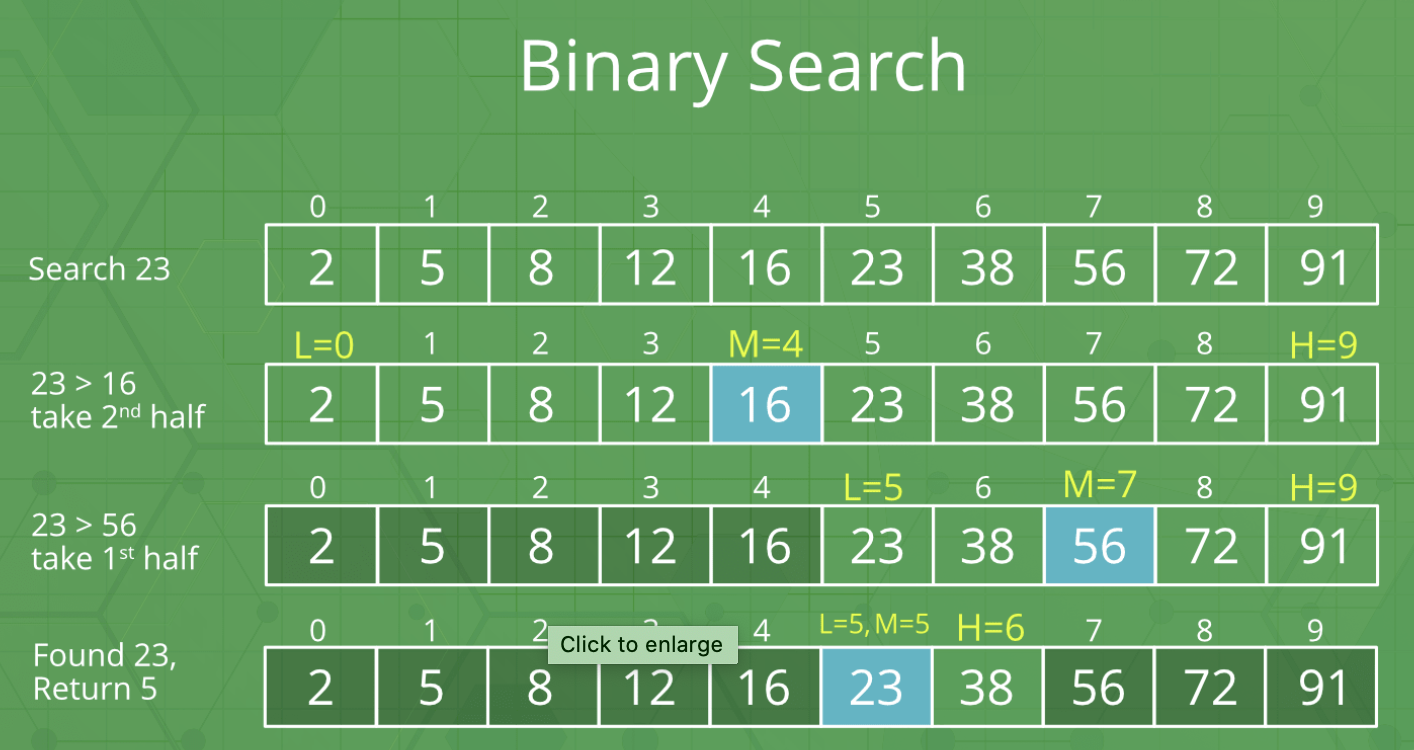
\includegraphics[width=\textwidth]{images/binary.png}
%     \caption{An example of using binary search to find number 23 in the given array. \href{https://www.geeksforgeeks.org/binary-search/}{\textit{Source}}}
%     \label{fig:binary}
% \end{figure}


% Below is an example implementation of binary search in Java.

% \begin{code}
% public class Example
% {
%     public static int binarySearch(int a, int b)
% 	{
% 	if (a-b == 1) return a;
%  	int middle = a + (a-b)/2;
% 	StdOut.print("Is the secret number greater than or equal to " + middle + "? ");
% 	if (StdIn.readBoolean())
% 		return binarySearch(middle, b);
% 	else
% 		return binarySearch(a; middle);
% 	}
% 	public static void main(String[] args)
% {
% int k = Integer.parseInt(args[0]);
% int n = (int) Math.pow(2, k);
% StdOut.println("Choose a secret number between 0 and " + (n-1));
% int guess = binarySearch(0, n)
% StdOut.println("The secret number is " + guess);
% }
% }
% \end{code}
 
 
%  Mathematically, we can show that $T(n) = lg n$ where $T(n)$ is the number of questions. This, the running time of binary search is logarithmic.

% \subsection{Binary search in a sorted array}
% An important application of binary search is when we would like to find a piece of information using a key to guide the search. For example, in the last century people would use a phone book to look up a person’s phone number. In this case, the elements are sorted by a key (i.e. a person’s name, sorted in alphabetical order). Nowadays, we can implement this searching process using binary search.



% \section{Insertion sort}

% Now, we would like to discuss a few of the most fundamental sorting algorithms. 
% Let’s start with a brute force algorithm known as \textit{insertion sort}. This algorithm mimics a method that people usually use to arrange hands of playing cards. Consider the cards one at a time and insert each into its proper place among those that have already been considered. Below is an example Java method that rearranges the strings in an array to put them in ascending order:

% \begin{code}
% public static void sort(String[] a)
% {
% 	int n = a.length;
% 	for (int i = 1; i < n; i++)
% 		for (int j = i; j > 0; j- -)
% 			if (a[j-1].compareTo(a[j]) > 0)
% 				exchange(a, j-1, j)
% 			else break;

% }
 
% \end{code}
 
 
%  At i-th iteration of the outer \textit{for} loop, the first I elements in the array are in sorted order; the inner \textit{for} loop moves a[i] into its proper position in the array. Note that the running time of insertion sort is sensitive to its input values. For example, if the input array happened to be already sorted, the running time of the program is linear. However, if the input array is in reversed order, then the running time is quadratic. There are many real-world applications for which insertion sort is quadratic, so we need to consider faster sorting algorithms.

% \begin{figure}
%     \centering
%     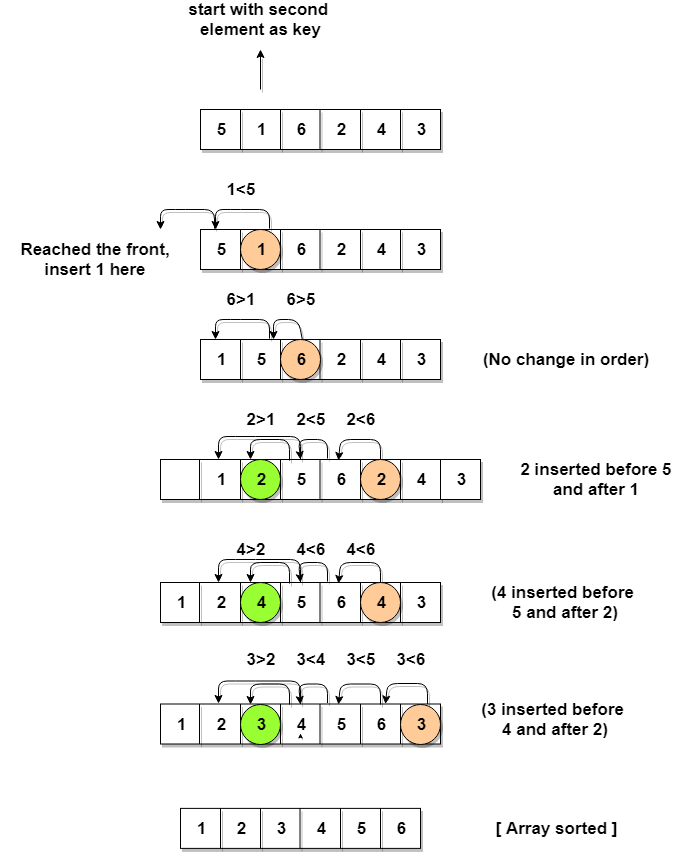
\includegraphics[width=\textwidth]{images/insertion-sort.png}
%     \caption{An example showing how the insertion sort algorithm works. \href{https://vivaharsha.com/product/verilog-implementation-of-insertion-sort-16-bits-and-5-inputs/}{\textit{Source}}}
%     \label{fig:insertion_sort}
% \end{figure}


% \section{Mergesort}
% To create a faster sorting method, we need to understand recursion and a \textit{divide-and-conquer} approach to algorithm design. \textit{Divide-and-conquer} approach refers to the idea that we can solve a problem by \textit{diving} it into in depend parts, \textit{conquer} them independently, and then use the solution for the parts to develop a solution to the original problem. Applying this approach to sorting, we can first divide an array into two halves, sort the two halves independently, and then \textit{merge} the results into the full array. This sorting algorithm is called \textit{mergesort}. 

% We consider contiguous subarrays of a given array \textit{array}, using the notation [a;b) to refer to the array consisting of elements array[a], array[a+1], …, array[b-1]. The mergesort algorithm implements the following strategy:
   
% \begin{itemize}
% \item \textit{Base case:} if the subarray length is 0 or 1, it is already sorted.
% \item \textit{Reduction step:} If not, compute $middle = a + (a+b)/2$, recursively sort the two subarrays array[a, middle) and array[middle, b] and merge them.
% \end{itemize}

% You can view a short video that shows an example of how the mergesort algorithm works \href{https://youtu.be/4VqmGXwpLqc}{\textit{here}}.




% \begin{exercise}

% Fill in the blanks in the implementation of the mergesort algorithm.
% \begin{code}

% public void merge(int[] list, int low, int high) {
% // temporary array stores the "merge" array within the method.

% int[] temp = new int[list.length];
%     // Set the midpoint and the end points for each of the subarrays
%     int mid = (low + high)/2;
%     int index1 = 0;
%     int index2 = BLANK ;
%     int index3 = mid + 1;
%     // Go through the two subarrays and compare, item by item,
%     // placing the items in the proper order in the new array
%     while (index2 <= mid && index3 <= high) {
%         if (list[index2] < list[index3]) {
%             temp[index1] = list[index2];
%             index1++;
%             index2++;
% }
% else {
%             temp[index1] = BLANK;
%             index1++;
%             index3++;
% } }
%     // if there are any items left over in the first subarray, add them to
%     // the new array
%     while (index2 <= mid) {
%         temp[index1] = list[index2];
%         index1++;
%         index2++;
% }
%     // if there are any items left over in the second subarray, add them
%     // to the new array
%     while (index3 <= high) {
%         temp[index1] = list[index3];
%         index1++;
%         index3++;
% }
%     // load temp array's contents back into original array
%     for (int i=low, j=0; i<=high; i++, j++) {
%         list[i] = BLANK;
%     }
% }

 
% \end{code}
 

% \end{exercise}
 
%  Mathematically, we can show that the running time of mergesort is linearithmic.
 
 
%  \section{Quicksort}
 
 
%  Another sorting divide-and-conquer algorithm is called \textit{quicksort}. It works by \textit{partitioning} an array into two parts and then sorting the parts independently. The main feature of this sorting algorithm is the partiotioning process, which rearranges the array to make three conditions hold:

% \begin{itemize}
% \item The entry array[j] is in its final place in the array, for some j
% \item No entry in array[a] through array[j-1] is greater than array[j]
% \item No entry in array[j+1] through array[b] is less than array[j]
% \end{itemize}

% With this algorithm, we do the sorting by first partitioning the array and then applying this method recursively to the subarrays of the array. This algorithm shuffles the array before sorting it. 

% \textbf{Partitioning} To implement the quicksort algorithm, we first need to implement the partitioning method. First, we arbitrarily choose array[a] to be the partitioning item, which will go into its final position. Next, we search from the left end of the array for an entry that is greater than or equal to the partitioning item. We then search from the right end of the array for an entry that is less than or equal to the partitioning item.The two found items are out of place so we exchange them. When the scan indices cross, to finish the partitioning process we need to exchange the partition item array[a] with the rightmost entry of the left subarray (array[j]) and return its index j.



% You can view a short video that shows an example of how the quicksort algorithm works \href{https://youtu.be/Hoixgm4-P4M}{\textit{here}}.

% \begin{figure}
%     \centering
%     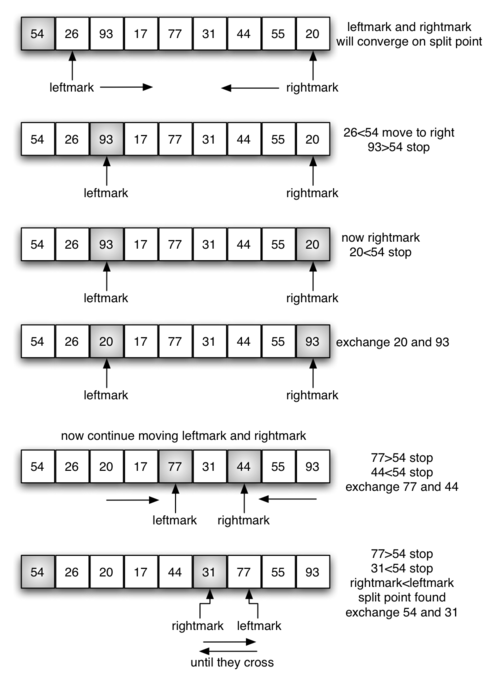
\includegraphics[width=\textwidth]{images/quicksort.png}
%     \caption{An example showing how the quicksort algorithm works. \href{https://runestone.academy/runestone/books/published/pythonds/SortSearch/TheQuickSort.html}{\textit{Source}}}
%     \label{fig:insertion_sort}
% \end{figure}


% \begin{exercise}
% Choose your favorite searching or sorting algorithm and run experiments with different input sizes to determine how the running time of the program changes with the input size. Run the algorithms on ten different input sizes and make a plot of the running time as a function of the input size.

% \end{exercise}